\chapter{Chromaticity in the FFS}\label{s:FFS}
\section{Chromaticity minimization in the Final Doublet (FD)}\label{s:chromFD}
% \section{Thin lens approximation}
In this Section I find the Final Doublet distance that minimizes the chromaticity.\par 
In the thin lens approximation, an FD as in Fig.~\ref{f:FDchrom}, with $r=L/L_{IP}$ and $r_{im}=L_{IM}/L_{IP}$, has peak $\beta$-functions at the quadrupoles equal to $\beta_{\genfrac{}{}{0pt}{}{x0}{y0}}=\frac{L^2_{IP}}{\beta^*_{\genfrac{}{}{0pt}{}{x}{y}}}$  for $QD0$ and $\beta_{\genfrac{}{}{0pt}{}{x1}{y1}}=\beta_{\genfrac{}{}{0pt}{}{x0}{y0}}\left(1+r\pm\sqrt{\frac{r}{r_{im}}+r+\frac{r^2}{r_{im}}}\sqrt{\frac{1+r}{1+r/r_{im}}}\right)^2
$ for $QF1$, using $\left(\frac{\beta^*}{L_{IP}}\right)^2\ll1$, i.e. a small $\beta$ function far from QD0. The factor $\beta_{\genfrac{}{}{0pt}{}{x1}{y1}}/\beta_{\genfrac{}{}{0pt}{}{x0}{y0}}$ is the beta function at QF1 relative to QD0.\par
\begin{figure}[!htb]
 \centering
 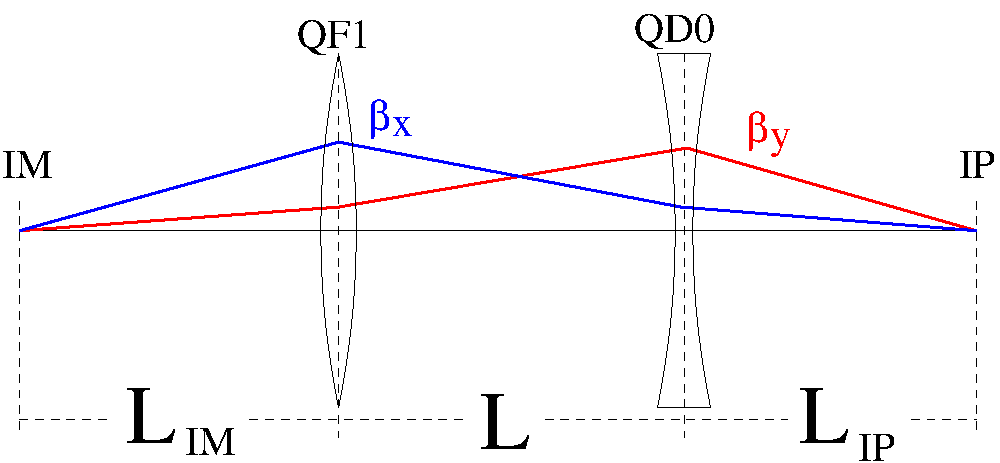
\includegraphics[scale=0.6]{fig01.pdf}\caption{FD with focal points IM and IP at different distances.}\label{f:FDchrom}
 \end{figure}
Being the chromaticity for a single quadrupole as in Eq.~(\ref{eq:chrom}) from~\cite{GarciaMorales:1982827}, 
\begin{equation}
%  \xi_x = \frac{1}{\beta_x^*}\left(\cancelto{0}{T_{116}^2}\beta_{x0}+T_{126}^2\frac{1}{\beta_{x0}}\right)\qquad
%  \xi_y = \frac{1}{\beta_y^*}\left(\cancelto{0}{T_{336}^2}\beta_{y0}+T_{346}^2\frac{1}{\beta_{y0}}\right)\label{eq:chrom}
\xi_{\genfrac{}{}{0pt}{}{x}{y}}=\int\beta_{\genfrac{}{}{0pt}{}{x}{y}}(s)k(s)ds\label{eq:chrom}
\end{equation}
where the $k$ is the quadrupole gradient and $s$ the longitudinal coordinate, then, $\xi_{\genfrac{}{}{0pt}{}{x}{y}}$ can be evaluated as
\begin{equation}
 \xi_{\genfrac{}{}{0pt}{}{x}{y}}=\mp\left(\beta_{\genfrac{}{}{0pt}{}{x1}{y1}}k_1l_1-\beta_{\genfrac{}{}{0pt}{}{x0}{y0}}k_0l_0\right)=\frac{L_{IP}}{\beta^*_{\genfrac{}{}{0pt}{}{x}{y}}\Xi_{\genfrac{}{}{0pt}{}{x}{y}}(r,r_{im}})
\end{equation}
where $k,l$ are the quadrupole gradient and length, $\beta^*$ is the $\beta$ function at the IP, the indexes indicate the quadrupole and 
%  \begin{align*}
%  \Xi_{x\atop y}(r,r_{im})=&\mp\sqrt{\frac{1}{rr_{im}}+\frac{1}{r}+\frac{1}{r_{im}}}\sqrt{\frac{1+r/r_{im}}{1+r}}\\ &\left[\left(1+r\pm\sqrt{\frac{r}{r_{im}}+r+\frac{r^2}{r_{im}}}\sqrt{\frac{1+r}{1+r/r_{im}}}\right)^2\right.\\
%  &\qquad\qquad\qquad\qquad\qquad\quad-\left.\left(\frac{1+r}{1+r/r_{im}}\right)\right]
% \end{align*}\par
{\scriptsize
\begin{equation}
 \Xi_{\genfrac{}{}{0pt}{}{x}{y}}(r,r_{im})=\mp\sqrt{\frac{1}{rr_{im}}+\frac{1}{r}+\frac{1}{r_{im}}}\sqrt{\frac{1+r/r_{im}}{1+r}} \left[\left(1+r\pm\sqrt{\frac{r}{r_{im}}+r+\frac{r^2}{r_{im}}}\sqrt{\frac{1+r}{1+r/r_{im}}}\right)^2\right.-\left.\left(\frac{1+r}{1+r/r_{im}}\right)\right]
\end{equation}}\par
Figure~\ref{f:figT} show the chromaticity $\Xi_x$ and $\Xi_y$ in $L_{IP}/\beta^*$ units, and the ratio of the $\beta$ functions at the quadrupoles.\par
% The IP beam size is increased by chromaticity as $\sigma^*_{x\atop y}=\sigma_{{x0\atop y0}}\sqrt{1+\xi^2_{x\atop y}\sigma_\delta^2}$, where $\sigma_0^2=\beta^*\epsilon$, valid for both transversal planes. Therefore, luminosity is approximately affected by the horizontal and vertical chromaticity as \par
% \begin{equation}
%  L\propto\frac{1}{\sigma_x\sigma_y}=\frac{1}{\sigma_{x0}\sigma_{y0}\sqrt{1+(\xi^2_x+\xi^2_y)\sigma_\delta^2+\xi_x^2\xi_y^2\sigma_\delta^4}}
% \end{equation}
In order to minimize the product of dispersion and sextupole strengths used to substract the quadrupoles chromatic effect, explained in Section \ref{s:chromcorr}, one possibility is to minimize the sum of the horizontal and vertical chromaticities, i.e. the total chromaticity to be corrected. Being the sum, 
\begin{align}
 \xi = \xi_x + \xi_y &= \frac{L_{IP}}{\beta^*_y}\left(\frac{\Xi_x(r,r_{im})}{\beta^*_x/\beta^*_y}+\Xi_y(r,r_{im})\right)\\
 &= \frac{L_{IP}}{\beta^*_y}\Xi(\beta^*_x/\beta^*_y,r,r_{im})
\end{align}
Figure~\ref{f:fig_3TeV} shows $\Xi$ for CLIC 3 TeV, $\beta^*_x/\beta^*_y=6.9\text{mm}/0.068\text{mm}=101$, and Fig~\ref{f:fig_500GeV} is the equivalent for CLIC 500 GeV \cite{CLICdes}, $\beta^*_x/\beta^*_y=8.0\text{mm}/0.1\text{mm}=80$.\par
Given $L_{IM}$, the minimum added chromaticity in the FD is found when $L$ is one to two times the distance to the IP. In addition, Figs.~\ref{f:fig_3TeV}-\ref{f:fig_500GeV} show the effect of scaling up the system. For example, starting at $L=L_{IP}$ and $L_{IM}=10L_{IP}$, it is clear that a system with $L=10L_{IP}$ and $L_{IM}=100L_{IP}$, will decrease the vertical chromaticity by increasing the horizontal chromaticity.
\begin{figure}
\begin{subfigure}{0.5\textwidth}
 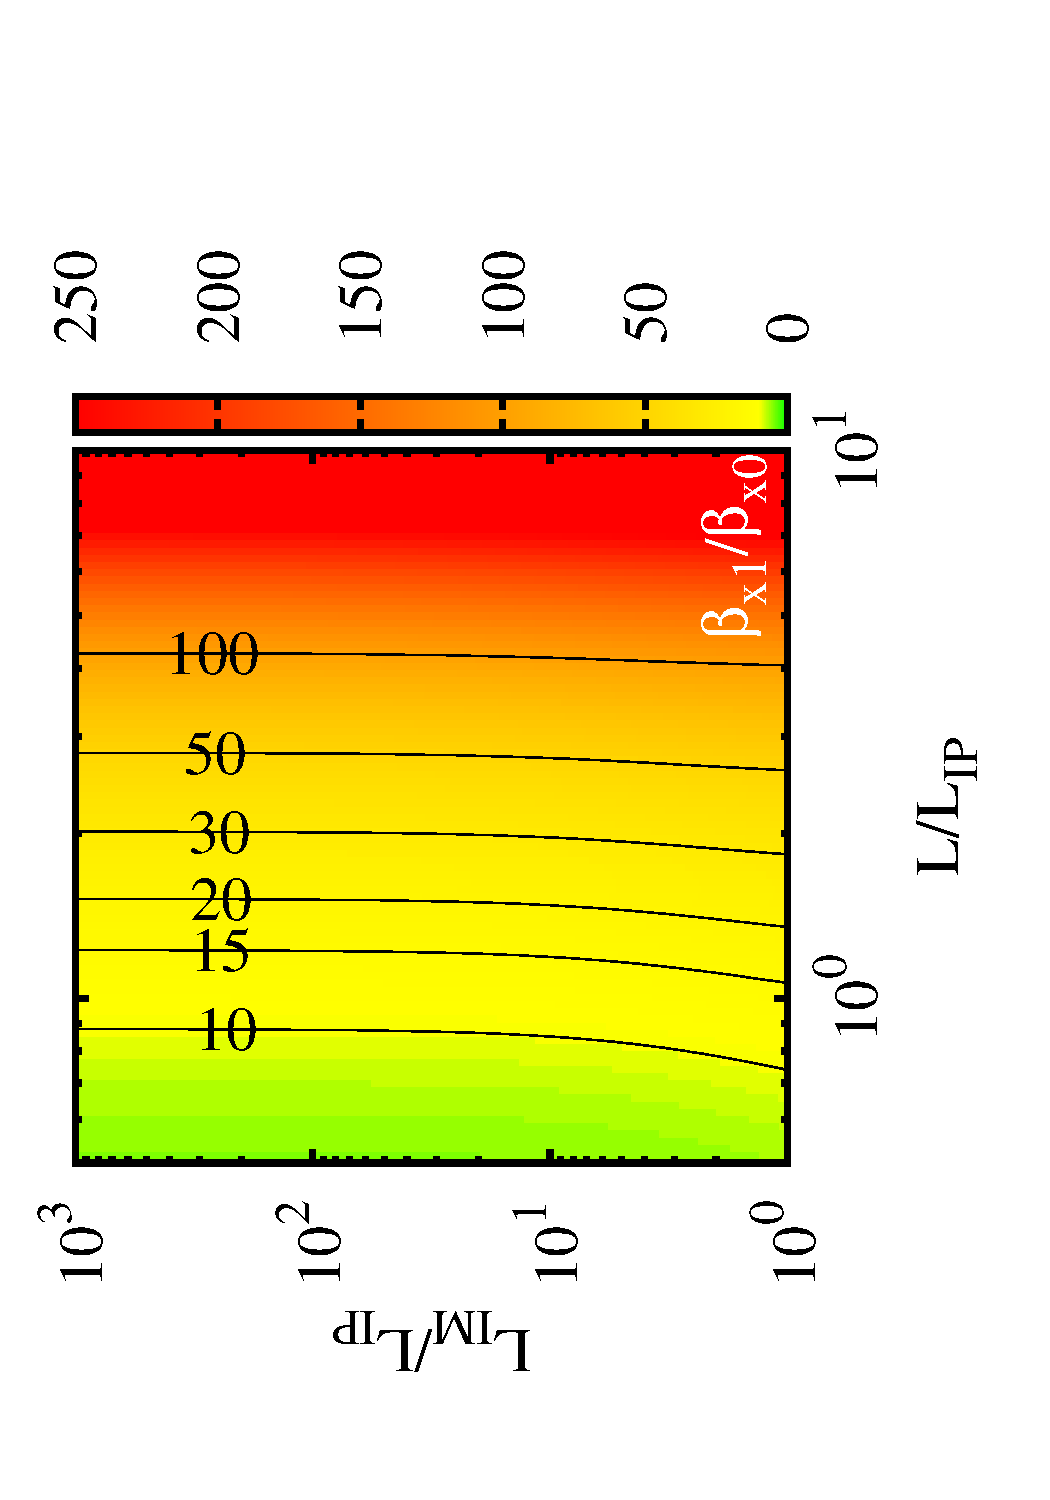
\includegraphics[scale=0.35,angle=-90]{./betax1a.pdf}\caption{}\label{figT:Bx}
 \end{subfigure}
 \begin{subfigure}{0.5\textwidth}
 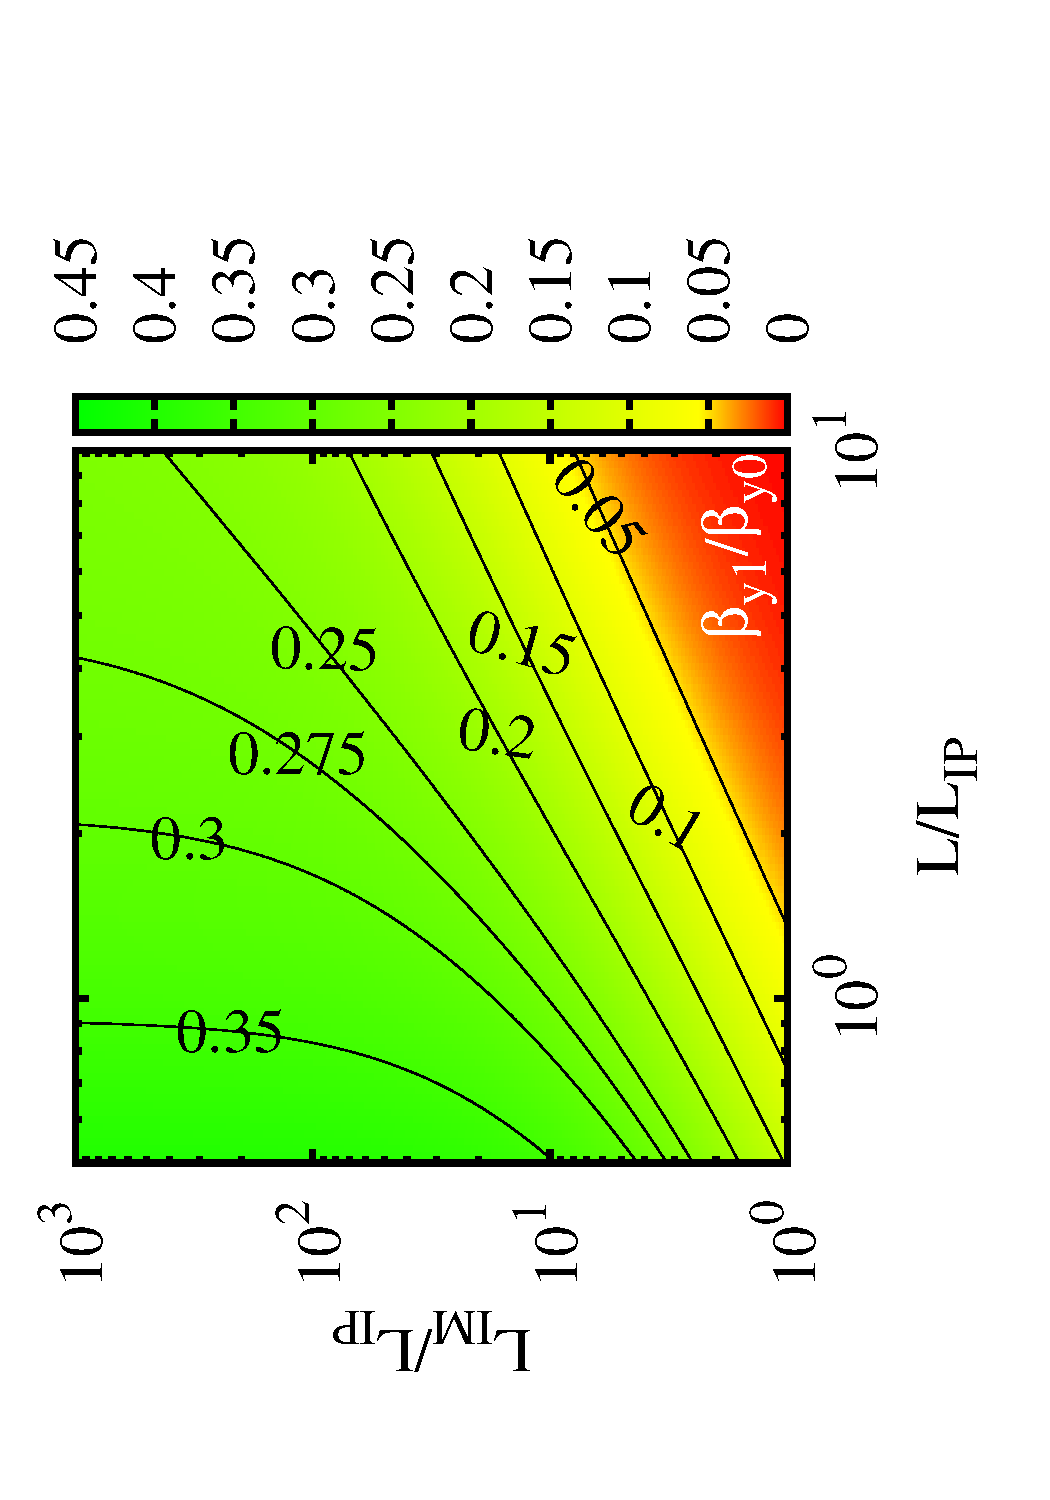
\includegraphics[scale=0.35,angle=-90]{./betay1a.pdf}\caption{}\label{figT:By}
 \end{subfigure}\\
 \begin{subfigure}{0.5\textwidth}
 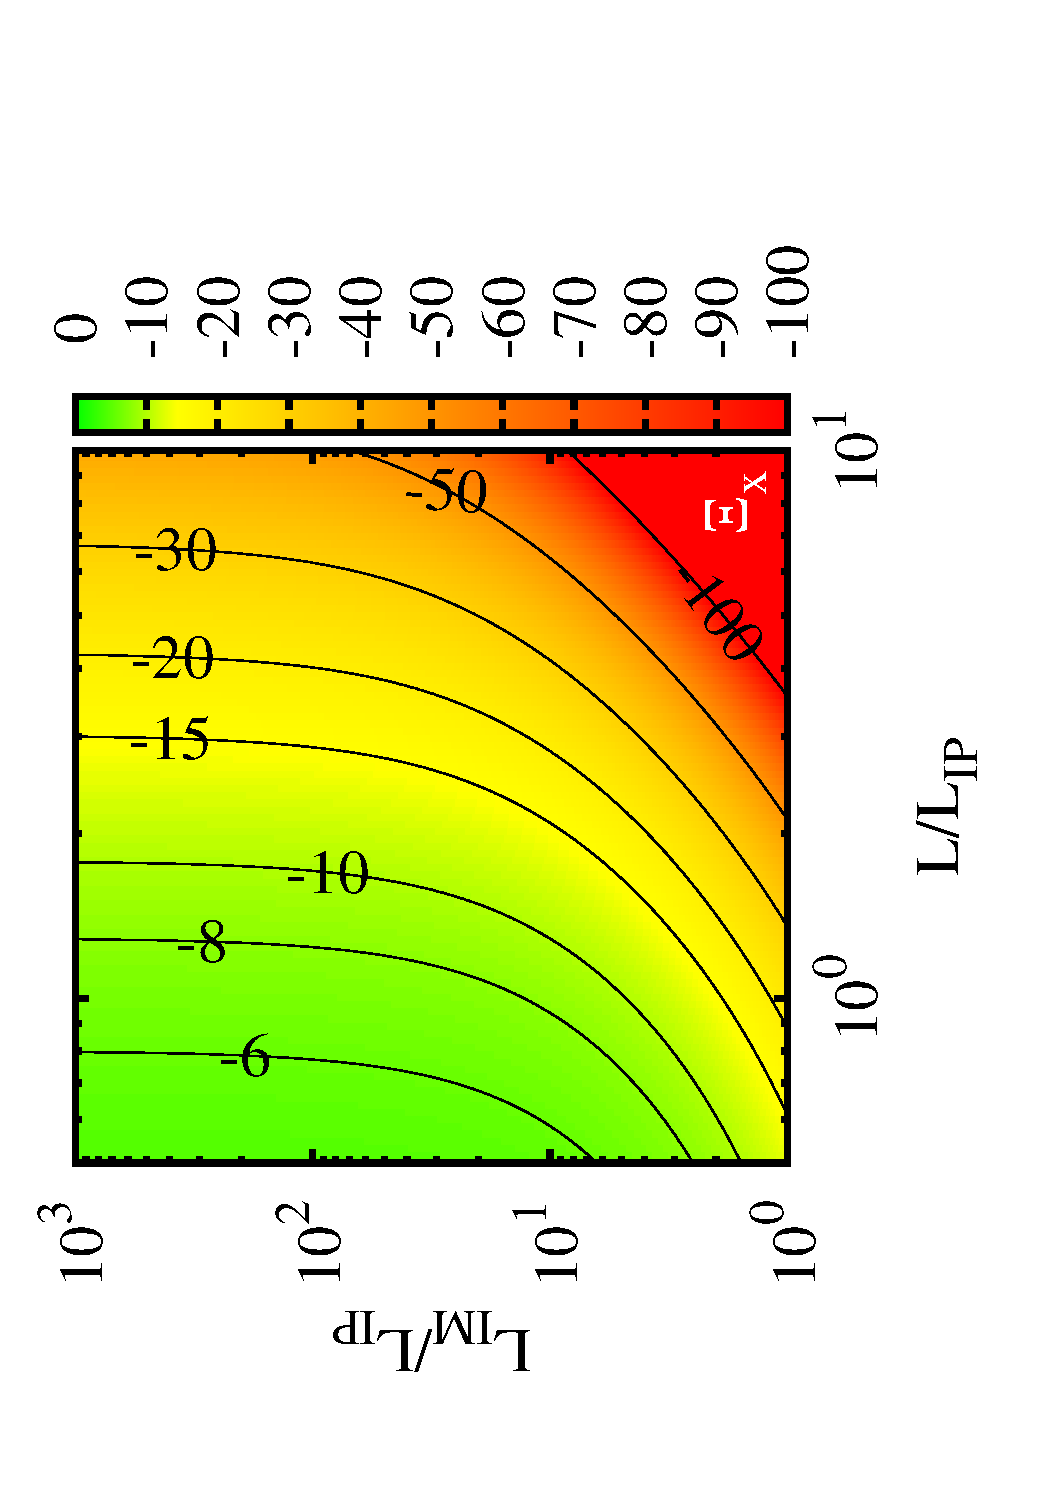
\includegraphics[scale=0.35,angle=-90]{./Xi_xa.pdf}\caption{}\label{figT:xix}
 \end{subfigure}
 \begin{subfigure}{0.5\textwidth}
 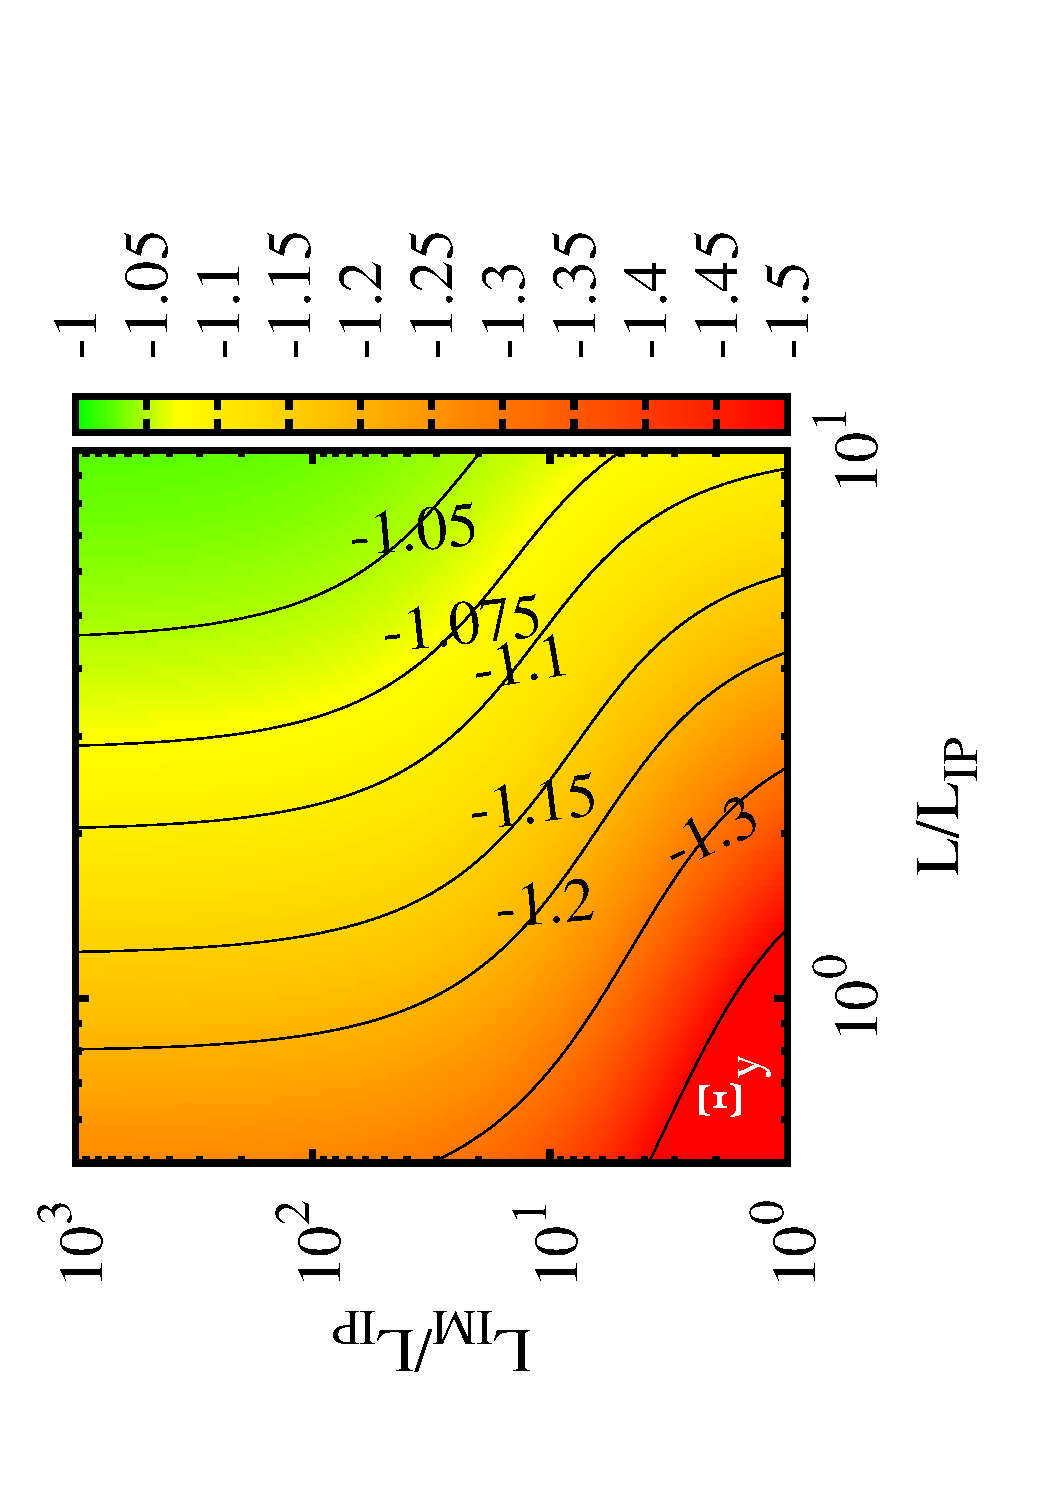
\includegraphics[scale=0.35,angle=-90]{./Xi_ya.pdf}\caption{}\label{figT:xiy}
 \end{subfigure}
 \caption{Normalized transversal functions (\ref{figT:Bx}) $\beta_{x1}/\beta_{x0}$, (\ref{figT:By}) $\beta_{y1}/\beta_{y0}$, (\ref{figT:xix}) $\Xi_x$, (\ref{figT:xiy}) $\Xi_y$}\label{f:figT}
\end{figure}
\begin{figure}
\begin{subfigure}{1.0\textwidth}
 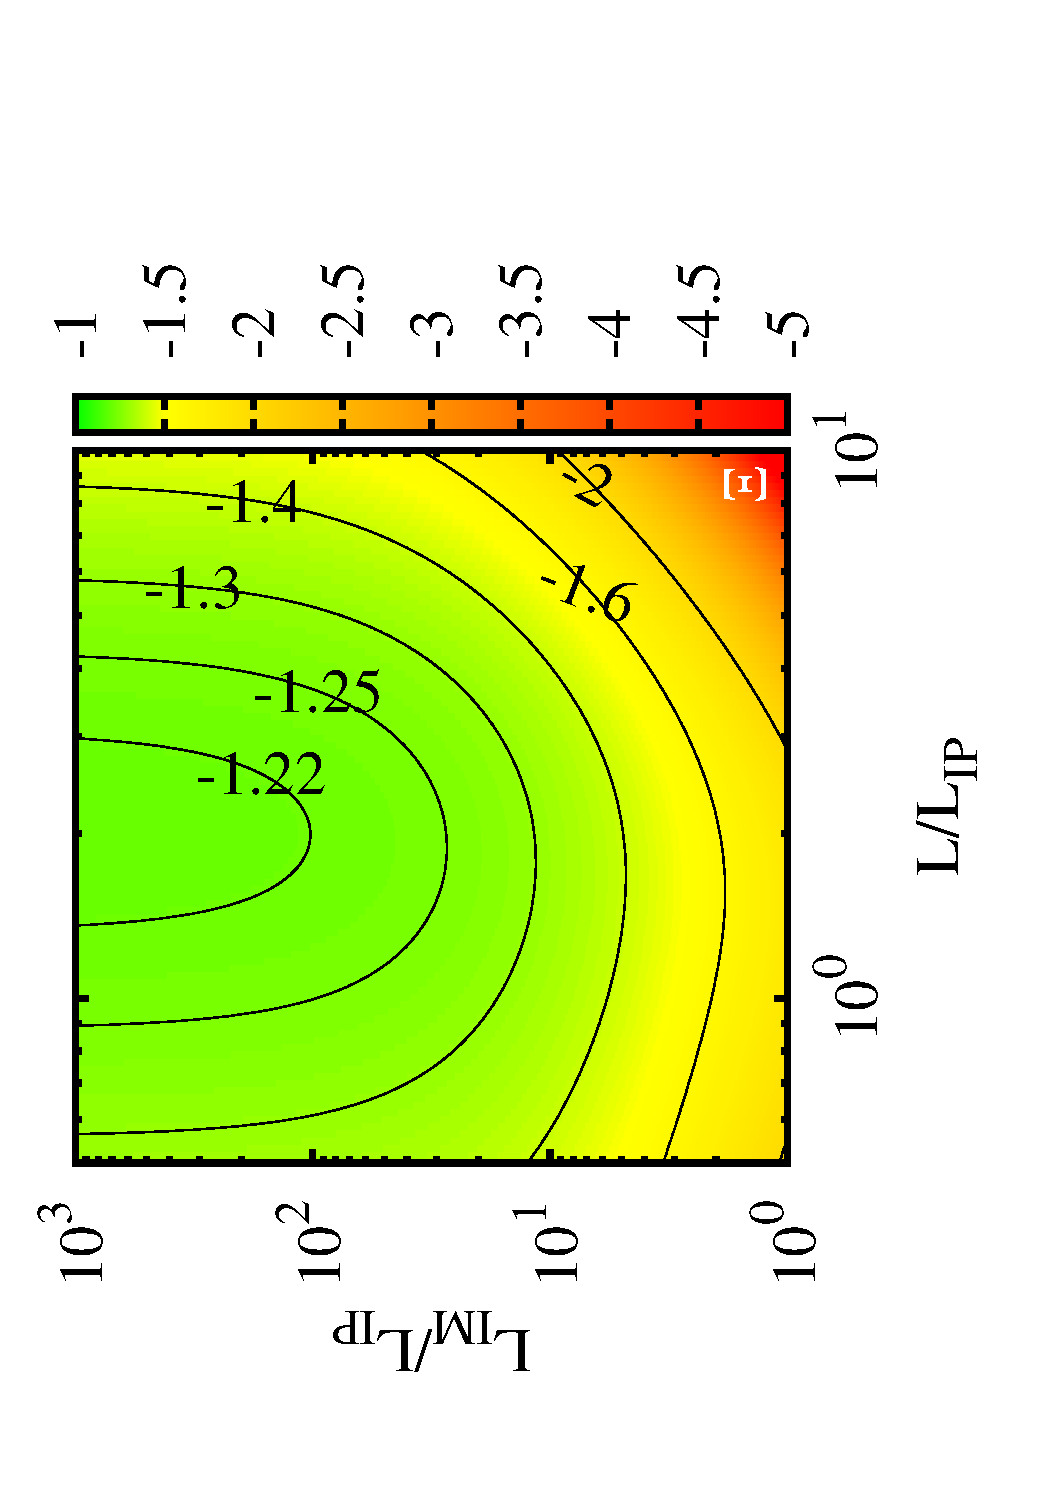
\includegraphics[scale=0.6,angle=-90]{./chromHV_3TeVa.pdf}\caption{}\label{fig_3TeV:chrom}
%  \includegraphics[scale=0.6,angle=-90]{./chromHV_500GeV.pdf}\caption{}\label{fig_chrom:b}
 \end{subfigure}\\
 \begin{subfigure}{0.5\textwidth}
 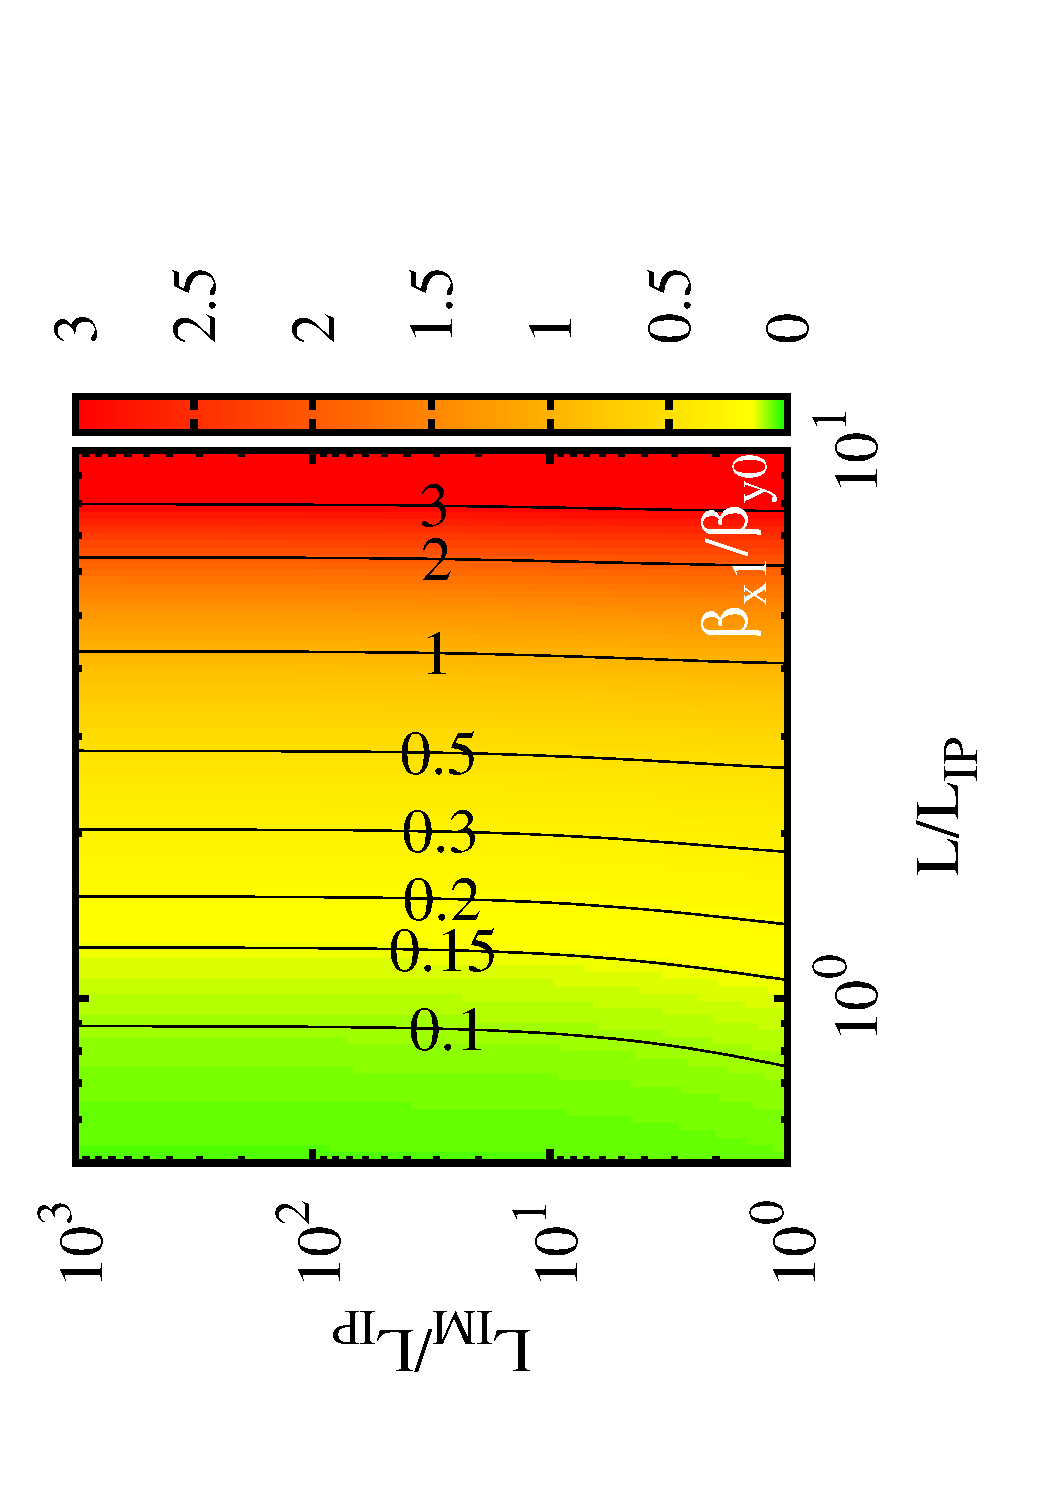
\includegraphics[scale=0.35,angle=-90]{./betax1_y0_3TeVa.pdf}\caption{}\label{fig_3TeV:bx1_y0}
 \end{subfigure}
  \begin{subfigure}{0.5\textwidth}
 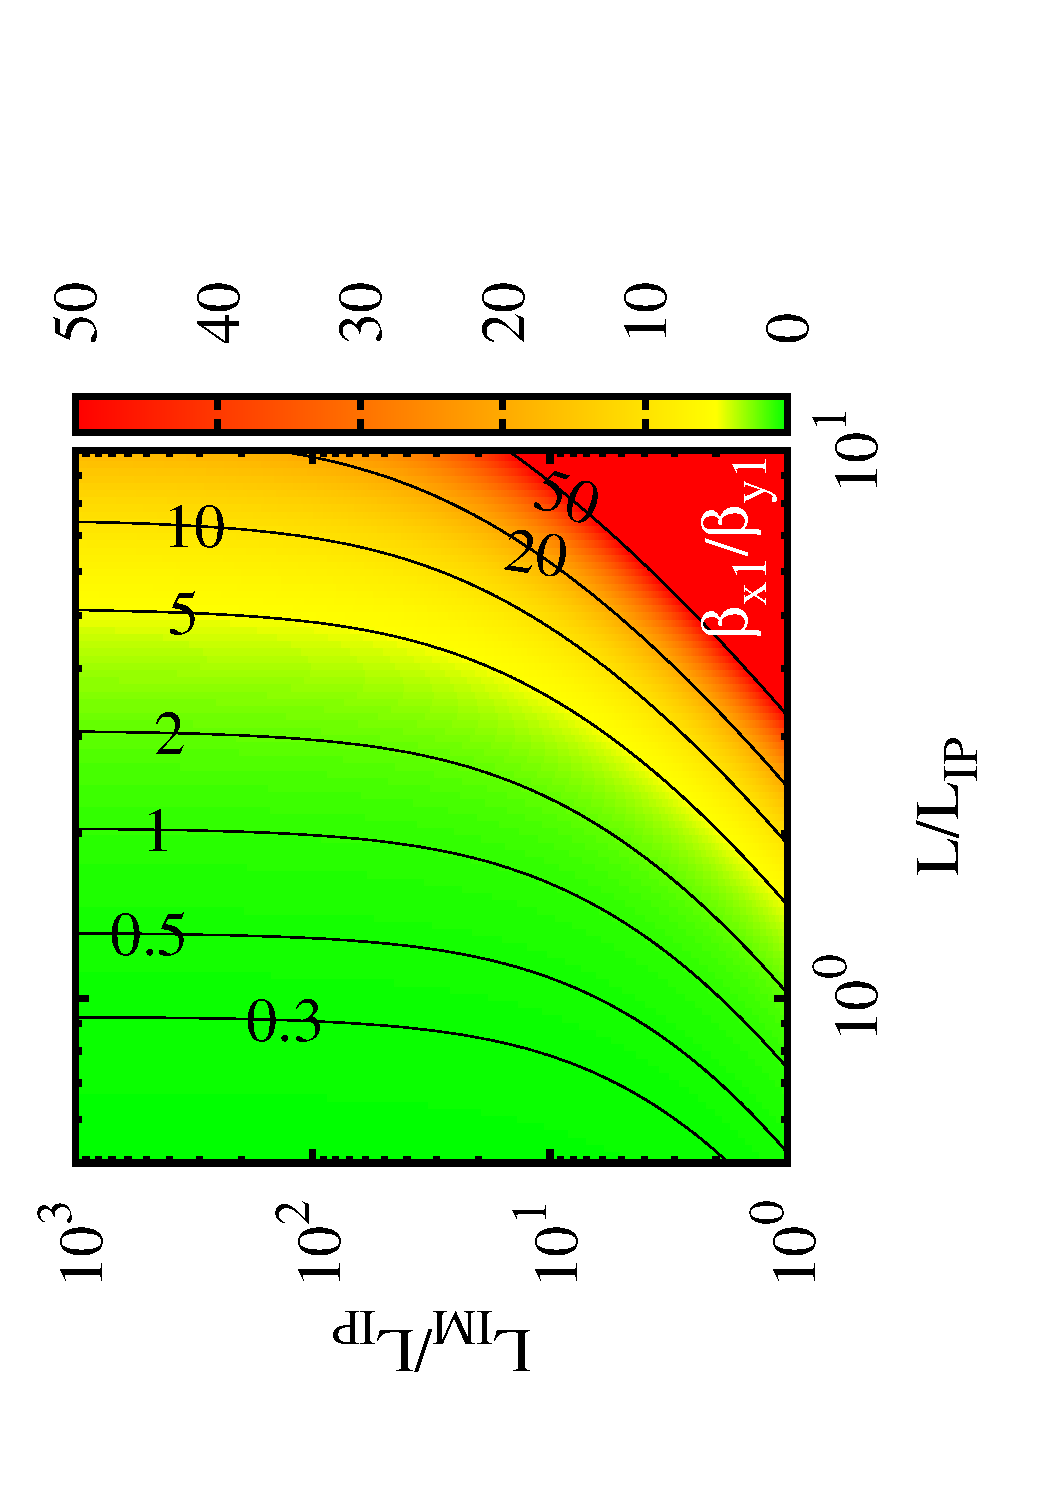
\includegraphics[scale=0.35,angle=-90]{./betax1_y1_3TeVa.pdf}\caption{}\label{fig_3TeV:bx1_y1}
 \end{subfigure}
 \caption{CLIC 3TeV (\ref{fig_3TeV:chrom}) $\Xi(\beta^*_x/\beta^*_y,r,r_{im})$, (\ref{fig_3TeV:bx1_y0}) $\beta_{x1}/\beta_{y0}$, (\ref{fig_3TeV:bx1_y1}) $\beta_{x1}/\beta_{y1}$}\label{f:fig_3TeV}
\end{figure}
\begin{figure}
\begin{subfigure}{1.0\textwidth}
%  \includegraphics[scale=0.6,angle=-90]{./chromHV_3TeV.pdf}\caption{}\label{fig_500GeV:chrom}
 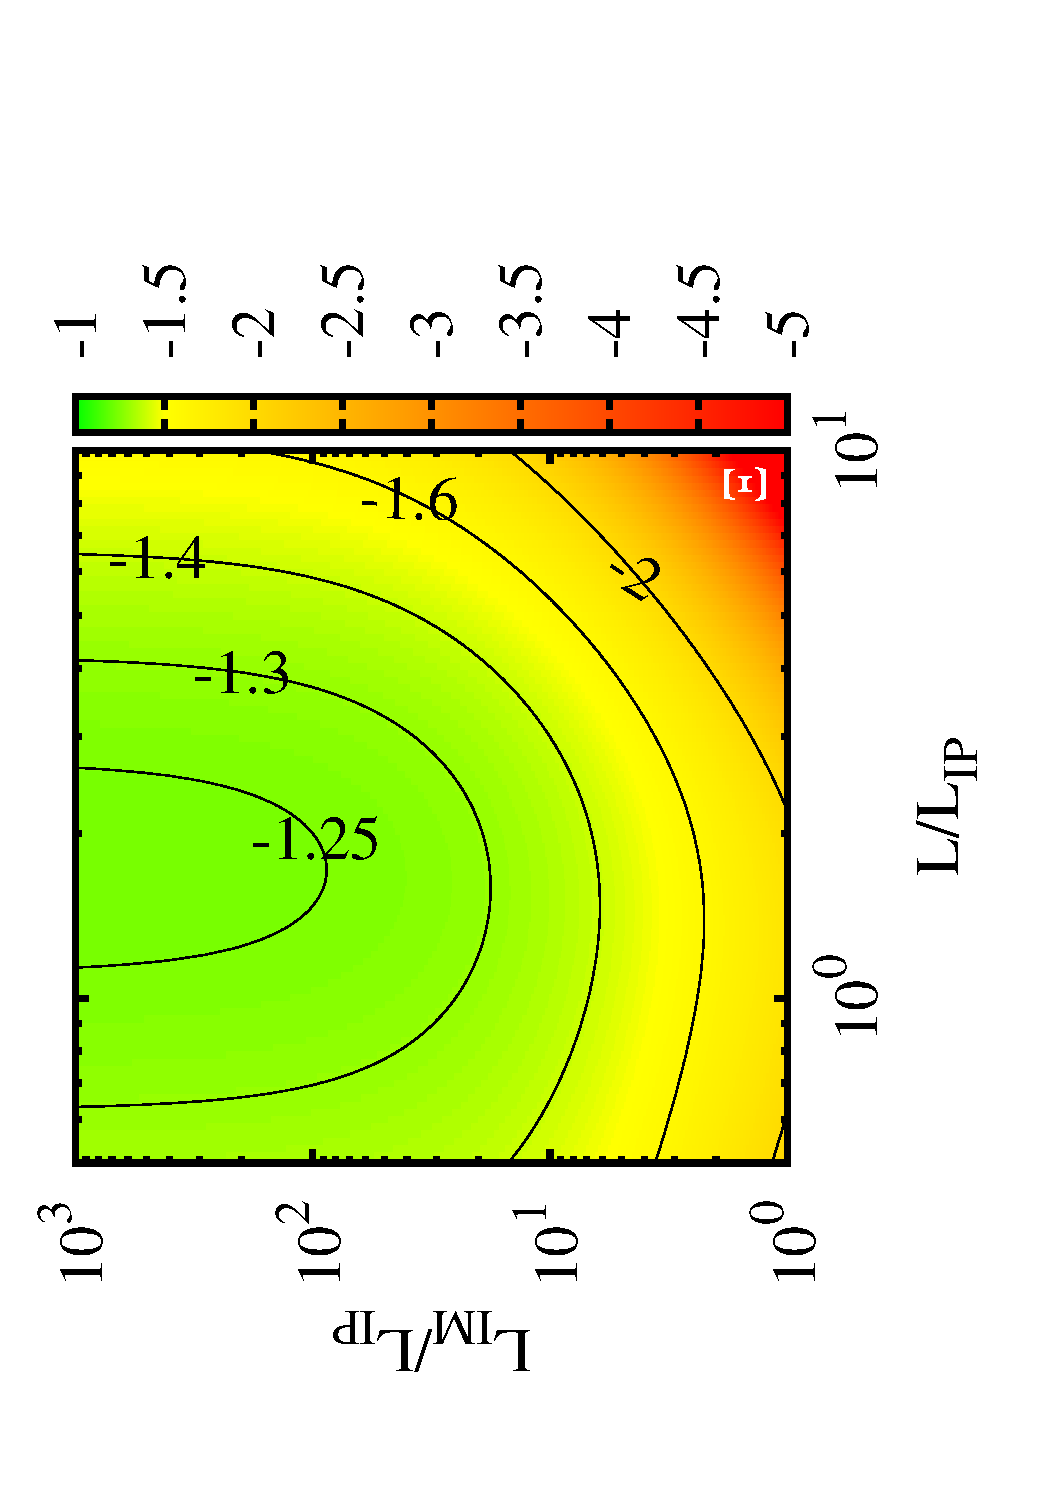
\includegraphics[scale=0.6,angle=-90]{./chromHV_500GeVa.pdf}\caption{}\label{fig_chrom:b}
 \end{subfigure}\\
 \begin{subfigure}{0.5\textwidth}
 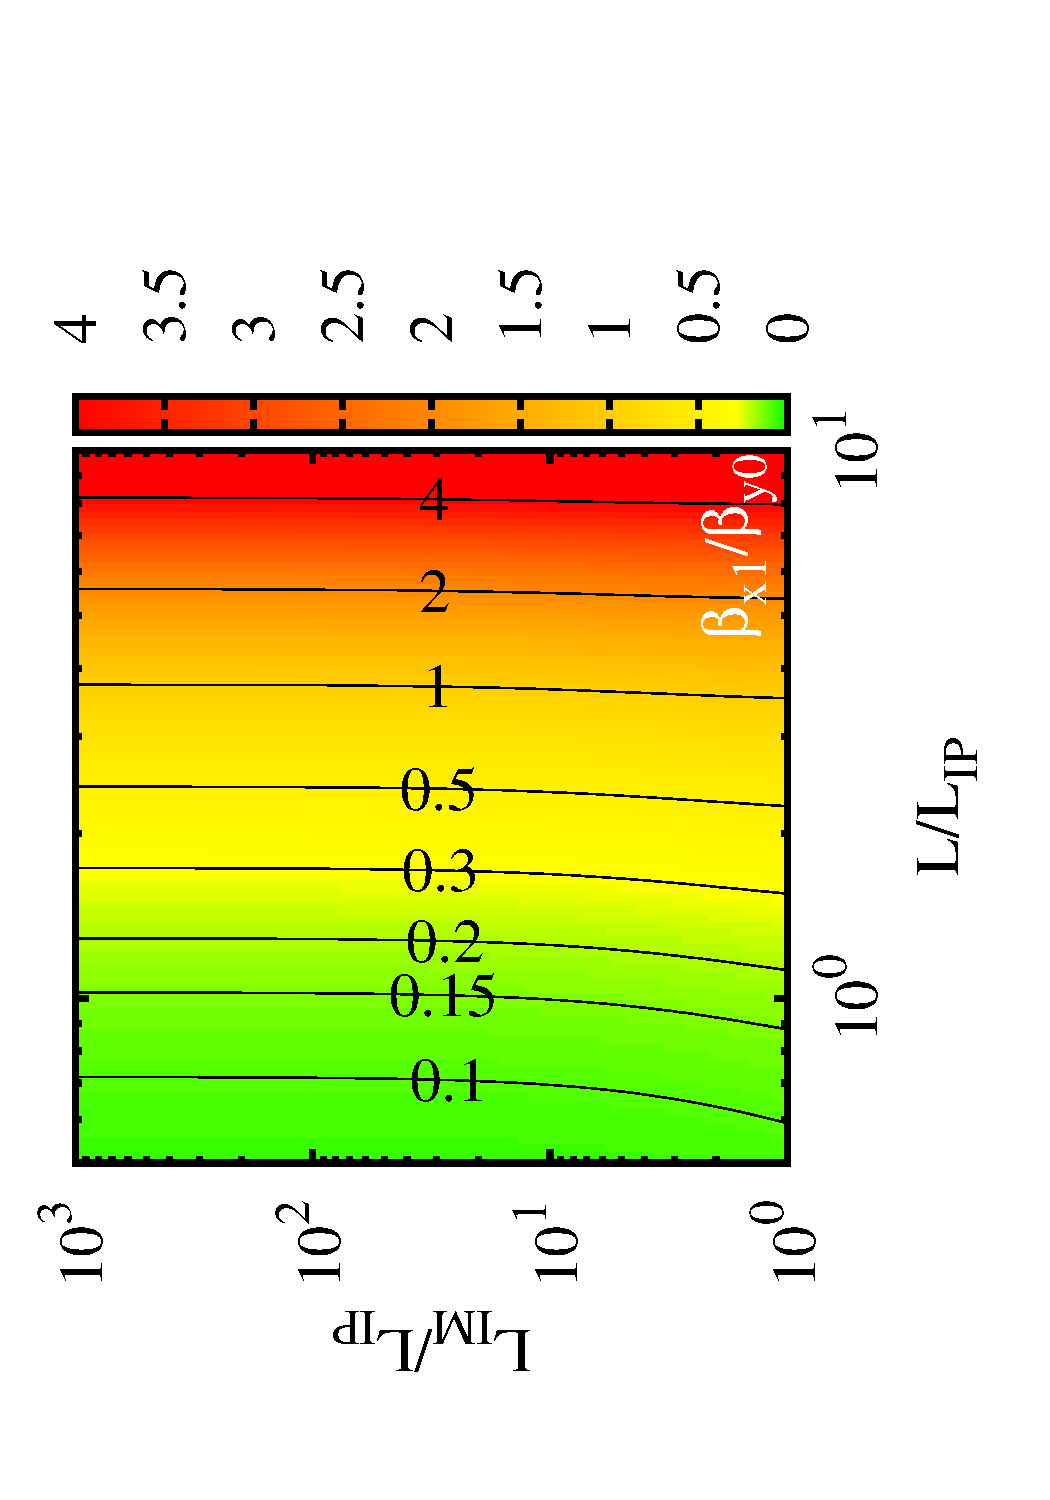
\includegraphics[scale=0.35,angle=-90]{./betax1_y0_500GeVa.pdf}\caption{}\label{fig_500GeV:bx1_y0}
 \end{subfigure}
  \begin{subfigure}{0.5\textwidth}
 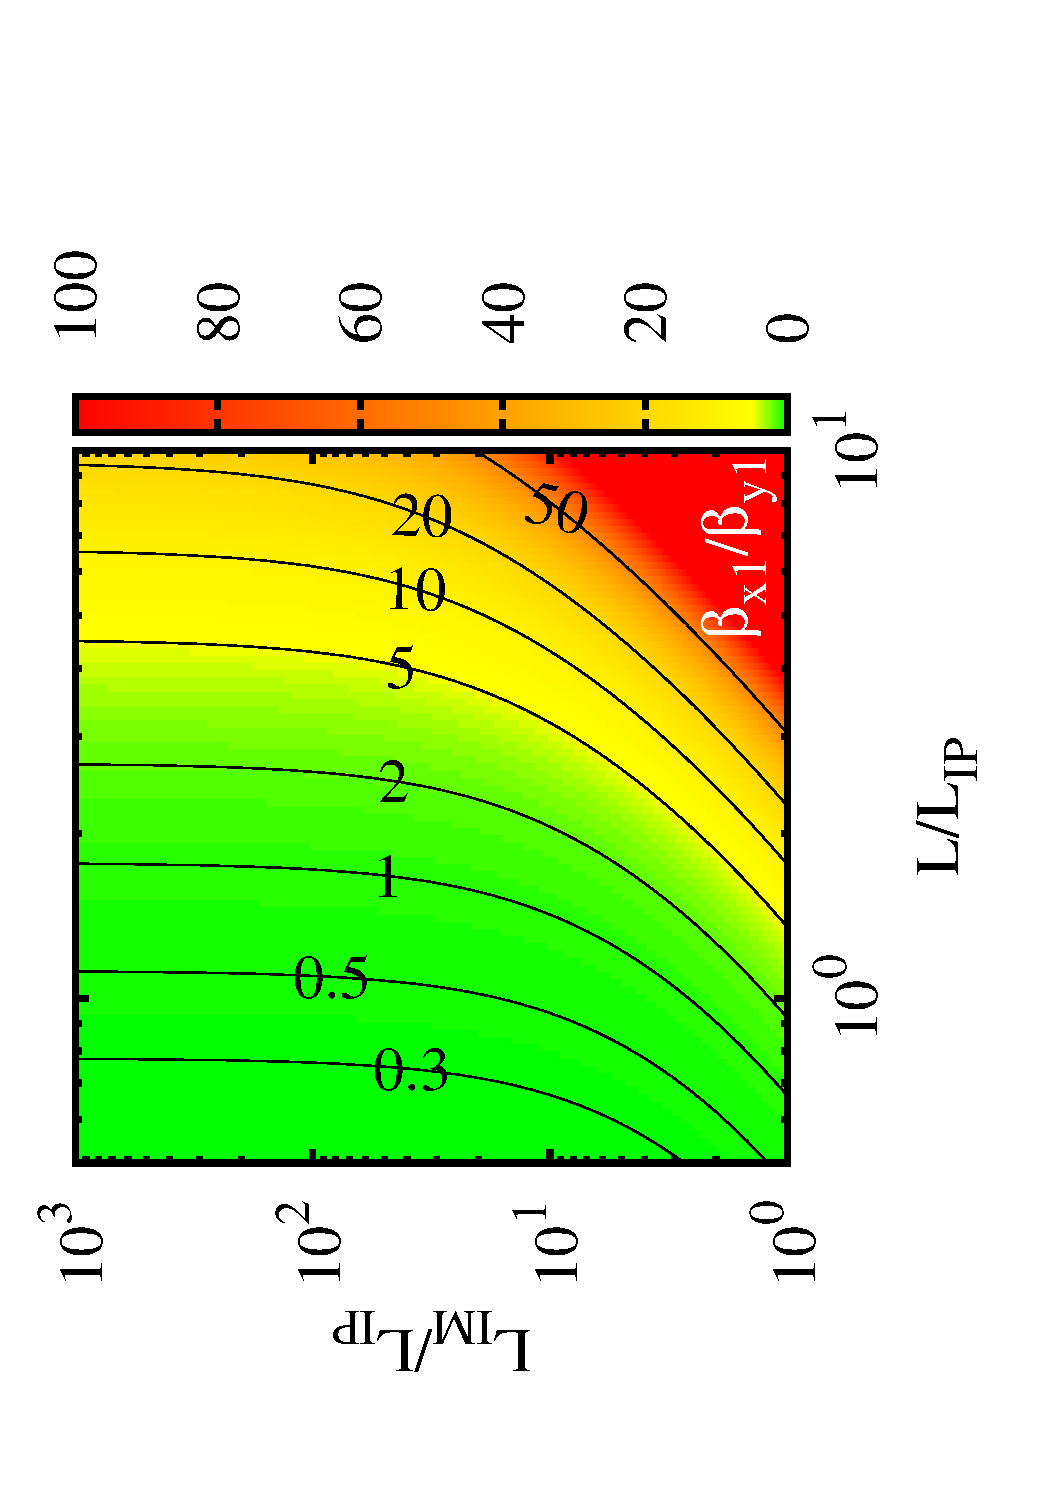
\includegraphics[scale=0.35,angle=-90]{./betax1_y1_500GeVa.pdf}\caption{}\label{fig_500GeV:bx1_y1}
 \end{subfigure}
 \caption{CLIC 500GeV (\ref{fig_3TeV:chrom}) $\Xi(\beta^*_x/\beta^*_y,r,r_{im})$, (\ref{fig_500GeV:bx1_y0}) $\beta_{x1}/\beta_{y0}$, (\ref{fig_500GeV:bx1_y1}) $\beta_{x1}/\beta_{y1}$}\label{f:fig_500GeV}
\end{figure}
\clearpage

\section{The non-interleaved lattice}\label{s:noninterleaved}
\subsection{Introduction}
Large chromaticity is generated in linear colliders due to the ratio of long $L^*$ and low-$\beta^*$ values. Table~\ref{t:chromlat} shows the chromaticity in the current three main linear collider projects.\par
\begin{table}[!htb]
% \scriptsize
\centering
\begin{tabular}{l|c||c|c|c}\hline
Parameter & Symbol & ILC & CLIC 500 GeV& CLIC 3 TeV\\\hline\hline
Distance from IP to QD0 [m] & $L^*$& 3.5/4.5 & 4.3 & 3.5\\
Vertical $\beta$ at the IP [mm] &$\beta_y^*$& 0.48 & 0.1&0.07\\
Energy Spread [$10^{-3}$]& $\delta$&3&3&3\\\hline
Vertical Chromaticity & $\xi_y\approx L^*/\beta^*_y$&7300/9400&43000&50000\\\hline
% Luminosity &$L$& $10^{34}$ &$1.57\times10^{34}$ & $2.3\times10^{34}$&$5.9\times10^{34}$\\\hline
\end{tabular}\caption{Approximative vertical chromaticity for the three current linear collider projects.}\label{t:chromlat}
\end{table}
Two methods have been used to cancel the chromatic effect: non-local and local correction. The local and non-local schemes, presented in Section~\ref{s:chromcorr}, have been compared for CLIC~\cite{PhysRevSTAB.17.101001}, concluding in easier tuning capabilities for the non-local. It has been mainly attributed to the separation of the horizontal and vertical chromatic correction sections, while in the local, the horizontal and vertical correction sections are interleaved.\par
% \subsection{The lattice}
This Section introduces an alternative lattice. In the non-interleaved scheme, the idea is to preserve the separation of the vertical and horizontal chromatic corrections  while cancelling the geometrical components in the vertical plane at the FD. One of the paired sextupoles is inside a horizontally dispersive region while the other remains outside to cancel geometric contributions.\par
\begin{figure}[!htb]
   \centering
   \includegraphics*[scale=0.2,angle=0]{noninterleavedcorr2.pdf}
   \caption{Non-interleaved chromaticity correction.}
   \label{f-noninterleaved}
\end{figure}
 Horizontal dispersion is generated over a common region and it is cancelled upstream, before the FD. Figure~\ref{f-noninterleaved} shows QD0 preceded by a sextupole SD0, which is matched with a second SD1 by the -I transport map. The same configuration is used to cancel horizontal chromaticity in an upstream section of the lattice using SF sextupoles.\par

 \subsection{Geometric Terms Cancellation}
Previously mentioned chromatic correction schemes use a pair of matched sextupoles to cancel one another geometrical components. It is generally noted as the -I transformation. However, results from \cite{PhysRevSTAB.8.104002} show that the -I transformation is one particular solution. When having a pair of sextupoles as in Fig.~\ref{f:sext} joined by a transport matrix $T_{12}$, the general solution for geometrical cancellation is
\begin{align}
t_{12}=&0\notag\\
t_{34}=&0\notag\\
t_{11}t_{22}=&1\notag\\
t_{33}t_{44}=&1\\
k_{s1}=&-k_{s2}t_{11}\notag\\
t_{11}=&\pm t_{33}\notag
\end{align}
where, $t_{ij}$ are the matrix elements and $k_{s1}, k_{s2}$ are the sextupole gradients. This general solution is used here to give more flexibility to the beta functions in the design. 
\begin{figure}[h]
   \centering
   \includegraphics*[scale=0.15,angle=0]{geo_cancel.pdf}
   \caption{Sextupoles joined by the transport matrix $T_{12}$.}
   \label{f:sext}
\end{figure}\par
Figure~\ref{f:phaseadv} shows the relative phase advances required in the non-interleaved design.
\begin{figure}[!htb]
   \centering
   \includegraphics*[scale=0.15,angle=0]{phase_adv.pdf}
   \caption{Phase advance in the non-interleaved lattice design.}\label{f:phaseadv}
\end{figure}\par
% \subsection{Tolerances}
Those expressions from the linear transport map set restrictions on the optic lattice parameters and tolerances during the lattice design stage. In order to evaluate those tolerances, $\Delta\phi_x, \Delta\phi_y, r_x, r_y$ have been defined as
\begin{align}
\phi_{x12}+\Delta\phi_{x} =& \pi\\
\phi_{y12}+\Delta\phi_{y} =& \pi\\
k_{s1}\beta_{x1}^{3/2}-k_{s2}\beta_{x2}^{3/2}+r_x=&0\\
k_{s1}\beta_{y1}^{3/2}-k_{s2}\beta_{y2}^{3/2}+r_y=&0
\end{align}
respectively, where $\Delta\phi$ is the phase advance error, $r$ is the residual after subtractions and $\phi,\beta$ are the optical parameters in horizontal $x$ and vertical $y$ planes for both sextupoles $S1$ or $S2$.\par
Factors $\alpha_{x1}\Delta\phi_x$, $\alpha_{x2}\Delta\phi_x$, $\alpha_{y1}\Delta\phi_y$, $\alpha_{y2}\Delta\phi_y\ll1$, with $\alpha$ the optic parameter, are conditions to achieve geometrical terms cancellation. The FD requires phase advances finely matched because $\alpha$ and $\beta$ are high, and the residuals $r_x,r_y$ should be close to zero in order to cancel the second order map components in both planes at the same time. The $\beta_y/\beta_x$ ratio can be chosen to match sextupole strengths.\par

\subsection{The Lattice}
Using the CLIC 500 GeV parameters listed in Table~\ref{t:CLIC500GeVnoninterleaved}, new lattices were designed in MAD-X~\cite{MADX} following the previous considerations and those in~\cite{Seryi-Raimondi2}. Figure~\ref{f:MAD-X} is an example. Phase advances have been matched to $10^{-6}$ precision due to high $\alpha$ values in the FD. MAPCLASS2~\cite{Mapclassorig,Mapclass,Mapclass2,githubMapClass2} gives vertical beam size of 1.9nm and horizontal beam size of 186nm to the first order.\par
\begin{table}[!htb]
\centering
 \begin{tabular}{l|c}\hline
  \textbf{Parameter, Symbol, [Units]} & \textbf{Value}\\\hline\hline
%   Length (linac exit to IP distance/side [m]) & 1750\\
  Maximum energy/beam, $E$, [TeV] & 0.25\\
  Distance from IP to first quad, $L^*$, [m] & 4.3\\
%   Crossing angle at the IP [mrad] & 18.6\\
  Nominal core beam size at IP, $\sigma^*$, $x/y$ [nm] & 202/2.3\\
%   Nominal beam divergence at IP, $\theta^*$, $x/y$ [$\mu$rad] & 25/23\\
  Nominal beta-function at IP, $\beta^*_x,\beta^*_y$, [mm] & 8/0.1\\\hline
%   Nominal bunch length, $\sigma_z$ [$\mu$m] & 72\\
%   Nominal disruption parameters, $D$, $x/y$ & 0.1/12\\
%   Nominal bunch population, $N$ & $6.8\times10^9$\\
%   Beam power in each beam [MW] & 4.9\\
%   Preferred entrance train to train jitter [$\sigma$] & $<0.2$\\
%   Typical nominal collimation aperture, $x/y$ [$\sigma_x/\sigma_y$] & 10/55\\
%   Vacuum pressure level, near/far from IP [$10^{-9}$ mbar] & 100/10\\\hline
 \end{tabular}\caption{CLIC 500 GeV parameters used for the non-interleaved lattice design.}\label{t:CLIC500GeVnoninterleaved}
\end{table}
\begin{figure}[!htb]
   \centering
   \hspace*{-0.6cm}
   \includegraphics*[scale=0.50,angle=0]{lattice_CLIC500_FF.pdf}
   \caption{Non-interleaved lattice design for CLIC 500 GeV. Dipoles in blue, horizontally focusing quadrupoles in red and above the axis, vertically focusing quadrupoles in red and below the axis, and sextupoles in black.}
   \label{f:MAD-X}
\end{figure}
However, Fig.~\ref{f-beamsize} shows that the horizontal beam size increases slightly to second order and by more than an order of magnitude when third order components in the map are considered.\par
\begin{figure}[!htb]
   \centering
   \hspace*{-0.6cm}
   \includegraphics*[scale=0.34,angle=0]{sigmas.pdf}
   \caption{Beam size at the IP of the CLIC 500 GeV non-interleaved design as a function of transfer map order obtained with MAD-X PTC.}
   \label{f-beamsize}
\end{figure}
The reason to this beam size growth is the second order dispersion ($T_{166}$) in the sextupole inside the FD, see Fig.~\ref{f-latticeT166}. As opposed to the local chromaticity method were $T_{166}$ is cancelled only at the IP by matching the sextupoles and dispersion function, here, the second order dispersion generates higher order components due to the sextupole inside the FD used for geometrical cancellation. This is not present in the non-local method because there is no sextupole in the FD.\par
Two possible solutions are foreseen at the moment : cancel the map components $T_{166}$ and $T_{266}$ before the FD, or alternatively tolerate some dispersion in the FD to cancel the second order map and making it similar to the local method.\par
\begin{figure}[!htb]
   \centering
   \hspace*{-0.6cm}
   \includegraphics*[scale=0.50,angle=0]{lattice_CLIC500_FF_T166.pdf}
   \caption{CLIC 500 GeV non-interleaved lattice. The second order dispersion from the $T_{166}$ map component is not zero at the sextupole in the FD.}
   \label{f-latticeT166}
\end{figure}
 
 \subsection{Conclusion}
The non-interleaved lattice proposal has been conceived as an alternative to the local and non-local chromaticity correction methods. The added horizontal and vertical chromaticity has been minimized by using a distance from QD0 to QF1 approximately one and two times the distance between QD0 and the IP. Also, a general geometrical cancellation has been used to give more flexibility to the linear lattice design, however the large beta functions close to the FD impose high precision in the phase advance betweeen sextupole elements.\par
The non-interleaved design for CLIC 500 GeV has been diagnosed using MAD-X and MAPCLASS2, concluding that the second order dispersion must be cancelled before the FD because of the high gradient sextupole before QD0 used to cancel geometrical components only.\par
Two solutions are foreseen : the cancellation of the second order dispersion and its derivative before the FD, or alternatively generate dispersion in the FD to cancel the residual second and third order components making it similar to the local correction.\par
Cancellation could be achieved by introducing an additional horizontal focal point upstream with no dispersion and no sextupole, this will increase the amount of total horizontal chromaticity, thereby changing the SF2 and SF3 sextupole strengths without changing the quads in the dispersive region, and enabling perhaps a better cancellation of T166 generated by the quad and sextupole in the dispersive part.% Playing with the magnitudes of the $\beta_x$ peaks at SF3 and SF2 will also change the amount of chromaticity to be corrected, but will not be efficient to improve the cancellation, as both terms (from the quads and SF2) will vary together.
